% das Papierformat zuerst
\documentclass[a4paper, 11pt]{article}

\usepackage[utf8]{inputenc} % Kodierung
\usepackage[ngerman]{babel} % Sprache
\usepackage{graphicx}  % Bildchen

% wir wollen auf jeder Seite eine Ueberschrift
\pagestyle{headings}

% hier beginnt das Dokument
\begin{document}

\thispagestyle{empty}
\begin{center}
\Large{Karlsruher Institut für Technologie}\\
\end{center}

\begin{center}
\Large{Fakultät für Wirtschaftswissenschaften}
\end{center}
\begin{verbatim}





\end{verbatim}
\begin{center}
\textbf{\LARGE{Seminararbeit}}
\end{center}
\begin{verbatim}


\end{verbatim}
\begin{center}
\textbf{am Institut für Angewandte Informatik und Formale Beschreibungsverfahren}
\end{center}
\begin{verbatim}


\end{verbatim}
\begin{abstract} Text der Zusammenfassung \end{abstract}
\begin{verbatim}









\end{verbatim}
\begin{flushleft}
\begin{tabular}{lll}
\textbf{Thema:} & & Linked Open Data basierte Web 3.0 Anwendungen \\
& & \\
& & \\
\textbf{eingereicht von:} & & Xinji Du, \flq{}jacobdu@hotmail.com\frq{}\\
& & Christoph Gielisch, \flq{}christoph.gielisch@web.de\frq{} \\
& & Andreas Gutzan, \flq{}andigutzan@gmx.de\frq{} \\
& & Clemens Stolle, \flq{}clemens.stolle@gmail.com\frq{} \\
& & \\
\textbf{eingereicht am:} & & 09. Juli 2011\\
& & \\
\textbf{Betreuer:} & & Herr Prof. Dr. Rudi Studer \\
& & Herr Dipl.-Wirt.-Ing. Daniel Herzig \\
& & Herr Dipl.-Inf. Benedikt Kämpgen \\
& & Herr Dipl.-Inf. Günter Ladwig
\end{tabular}
\end{flushleft}


\tableofcontents
\setcounter{page}{1}
\pagenumbering{Roman}
\newpage
% das Abbildungsverzeichnis
\listoffigures
\newpage


\setcounter{page}{1}
\pagenumbering{arabic}
\section{Einleitung}
\subsection{Problemdefinition}
\subsection{Herangehensweise und Ziele}
\newpage
\section{Beschreibung der Idee}
\subsection{Anwendungszenario}
Für die Anwendbarkeit des Programmes gilt es zunächst zwei verschiedene Grundüberlegungen zu separieren. Es stellt sich die Frage, welchen Nutzen das Produkt zum einen für den potentiellen Anwender, also den Spieler, und zum anderen für den Entwickler bzw. den Vertreibenden bietet.\\\\Für den Anwender ist das Programm ein Quiz- oder Lernspiel. Abgefragt werden hauptsächlich geografische Kenntnisse. Dabei sorgt eine Punktevergabe für einen kompetitiven Faktor. Das Spiel positionier sich somit sowohl als Edutainment-Software\footnote{Hier noch ne schöne Quelle hin} als auch als Unterhaltungssoftware für die kurzweilige Ablenkung, z.B. als Facebook-Spiel.\\\\Als Anbieter der Software ist neben der Schaffung einer Einnahmemöglichkeit über Werbeeinblendungen oder Verkauf der Software vor Allem die Generierung von strukturierten Daten interessant. 
\subsection{Spielablauf}
Der Spielablauf gliedert sich in zehn Fragerunden. In jeder Fragerunde sucht das Programm drei Fotografien zu einer europäischen Stadt, die gewissen Ansprüchen genügen muss\footnote{Verweis auf Filterbeschreibung in Kap.4}, heraus. Der Spieler muss nun versuchen diese Stadt mit Hilfe der Fotografien zu erkennen und sie auf einer Europakarte mit einem Mausklick möglichst genau zu lokalisieren. Er bekommt dabei weniger Punkte je weiter sein Tipp vom richtigen Zielort entfernt liegt, wobei ab einer gewissen Entfernung pauschal null Punkte vergeben werden.\\\\ Weiterhin kann er sich nach Bedarf in jeder Fragerunde im Tausch gegen Punkte drei neue Fotografien oder auch einen 200 Zeichen langen Kurzhinweis anzeigen lassen. Wenn der Spieler mit seinem Tipp eine gewisse Maximalentfernung nicht überschreitet bekommt er darüber hinaus eine Bonusfrage zur aktuellen Stadt oder deren Land gestellt. Diese vermittelt zusätzliche Hintergrundinformationenund gibt dem Spieler die Möglichkeit ein paar Bonuspunkte zu erspielen.\\\\ Die so in einer Fragerunde erspielten Punkte werden kumuliert. Ziel des Spiels ist es nach zehn Fragenrunden einen möglichst hohen Punktestand zu erreichen.
\subsection{Alleinstellungsmerkmal und Abgrenzung}
Die grundlegende Spielidee wurde so schon in Facebook- sowie iPhone-Apps implementiert\footnote{Hier noch ein paar Namen bzw. Beispiele nennen}. Allerdings setzen diese zur Erzeugung der Fragen auf statische Datenbanken und sind somit im Fragenumfang limitiert. Durch den Einsatz von Linked-Open-Data konnte hier eine dynamische, sich selbstständig aktualisierende Variante geschaffen werden. Desweiteren sorgt der Aufbau des Programmes, gerade in Bezug auf die Bonusfragen, für eine modularisierte Erweiterbarkeit des bestehenden Programmes mit anderen Datenquellen im Semantic Web.\\\\Dazu kommt, dass das Programm keinerlei Anforderungen an den Nutzer stellt, wie die Wahl eines geeigneten Betriebssystems oder einen eingerichteten Account auf der Website. Lediglich ein aktueller Browser wird benötigt.
\subsection{Semantic Gaming}
\newpage
\section{Projektplanung}
\subsection{Ablauf der Planung}
\subsection{Arbeitspakete und Zuständigkeiten}
\newpage
\section{Umsetzung, Softwarepakete und Programm}
\subsection{Schematischer Aufbau, Konzeptskizze}

\begin{figure}
	\centering
	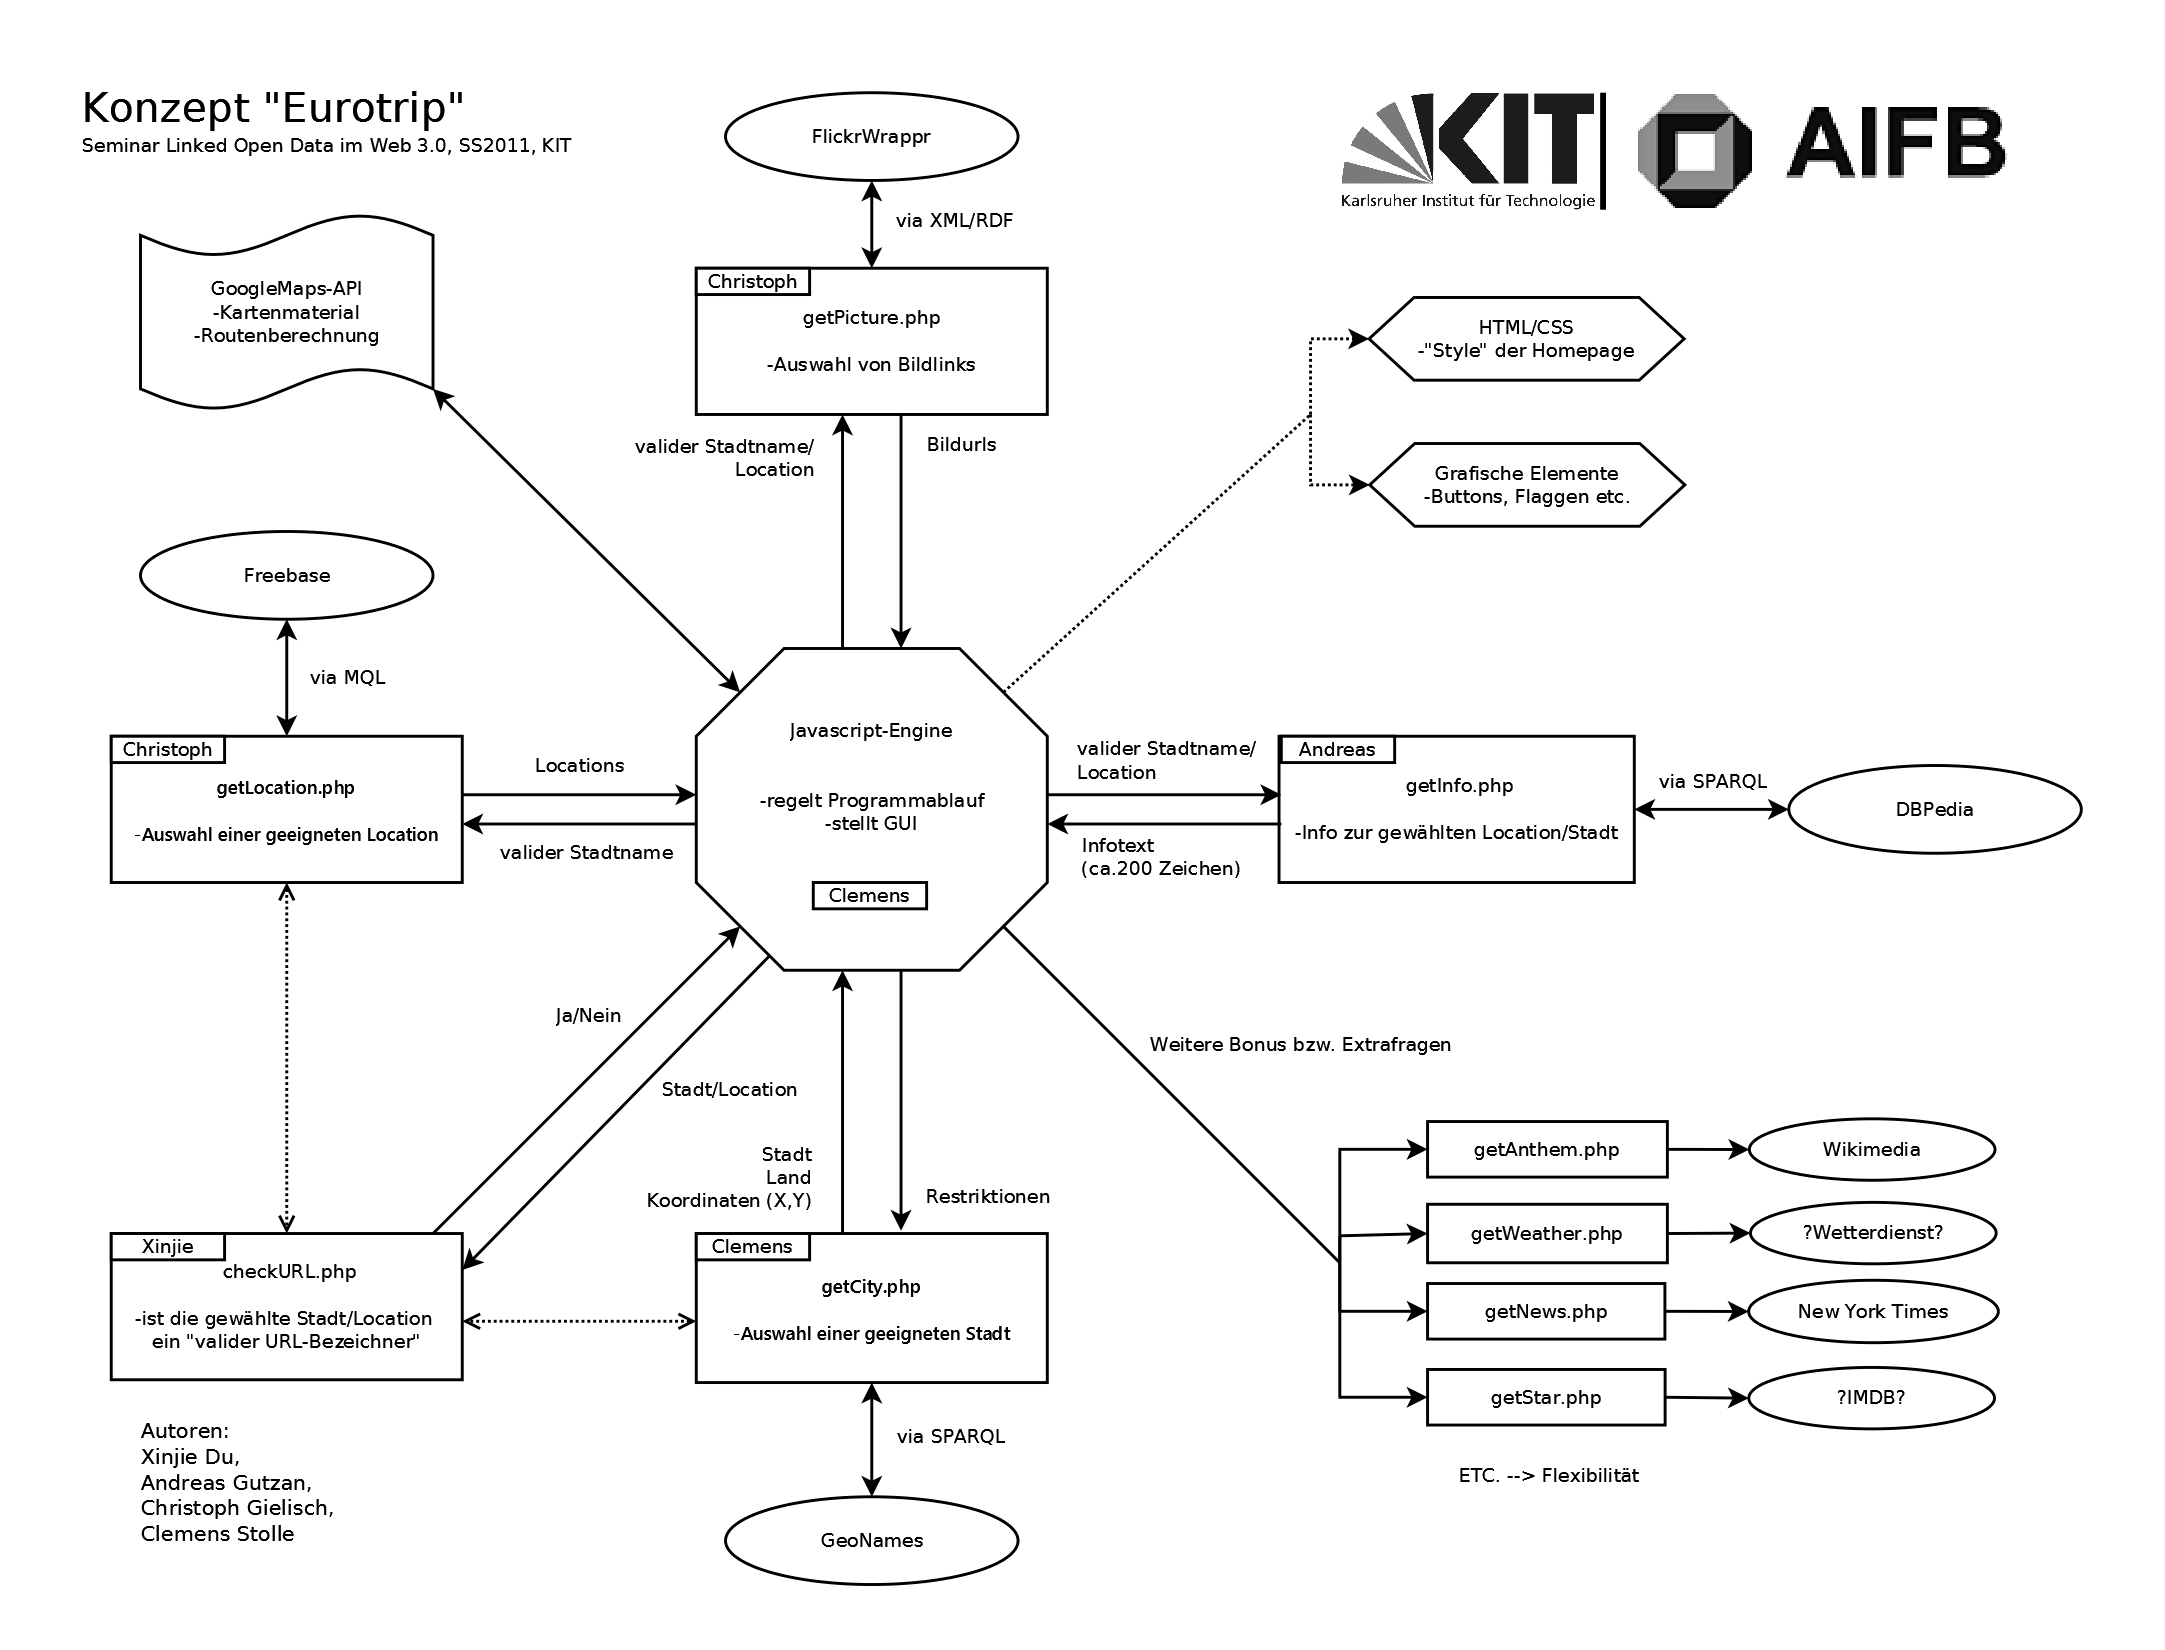
\includegraphics[width=1.4\columnwidth, angle=90]{seminarLOD.png}
	\caption{Konzeptskizze}
	\label{img:grafik-dummy}
\end{figure}

\subsection{Verwendete LOD-Datensätze}
Die verwendeten LOD-Datensätze sind:
\begin{itemize}
\item \textbf{Geonames}
\item \textbf{DBpedia}
\item \textbf{Freebase}
\item \textbf{Flickrwrappr}
\item \textbf{Weitere (Bonusfrage)}
\end{itemize}
\subsection{Verwendete Technologien und Frameworks}
Neben dem Linked-Open-Data Ansatzes des Semantic Webs benutzt das Programm selbst noch weitere Frameworks.
\subsection{Dokumentation der Methoden und Funktionen}
\subsection{Stabilität und Verfügbarkeit}
Das Programm an sich läuft trotz seines Prototypen-Status recht stabil. Allerdings ist die Erreichbarkeit von drei Datenquellen für den grundlegenden Ablauf der Fragerunden zwingend erforderlich. Diese sind Geonames, die DBpedia sowie der Flickrwrappr. Ein Ausfall der Freebase würde lediglich die Qualität der Bilder senken, da dann das Heraussuchen von Touristischen Attraktionen wegfallen würde. Sollte einer der Datenbanken der Bonusfragen nicht antworten, wäre ein Fallback auf eine andere Bonusfrage oder das komplette Deaktivieren denkbar. Bei beiden Möglichkeiten ist weiterhin ein stabiler, wenn auch eingeschränkter Betrieb des Programms möglich.\\\\ // Hier noch etwas zur Verfügbarkeit der einzelnen Datenquellen
\subsection{Installation und Betrieb}
Das Spiel selbst benötigt keine clientseitige Installation. Einzig ein funktionierender, aktueller Browser, der in der Lage ist Javascript auszuführen, ist von Nöten. Der Start erfolgt durch Ansteuerung der Webadresse.\\\\Für den Betrieb des Spiels ist der Anbieter des Porgramms allerdings gezwungen einen Webserver zu betreiben. Dieser muss in der Lage sein PHP-Code zu interpretieren und so die nötigen Abfragen auf die verschiedenen Datenquellen auszuführen.
\newpage
\section{Lessons learned}
\subsection{Reflektion der Projektplanung}
\subsection{Erkenntnisse}
\subsection{Vor- und Nachteile von Linked Open Data}
\newpage
\section{Fazit}
\subsection{Zusammenfassung}
\subsection{Stärken und Schwächen}
\subsection{Ausblick}

  
% das ist wohl jetzt das Ende des Dokumentes
\end{document}